\clearpage
\subsection{Expression} % (fold)
\label{sub:expression}

Some statements need data, this data can be calculated or provided as a literal value in the code. The term \textbf{expression} is used in programming to describe the places in a statement where data must be supplied. At run time each expression becomes a value that is used by the statement.

\begin{figure}[h]
   \centering
   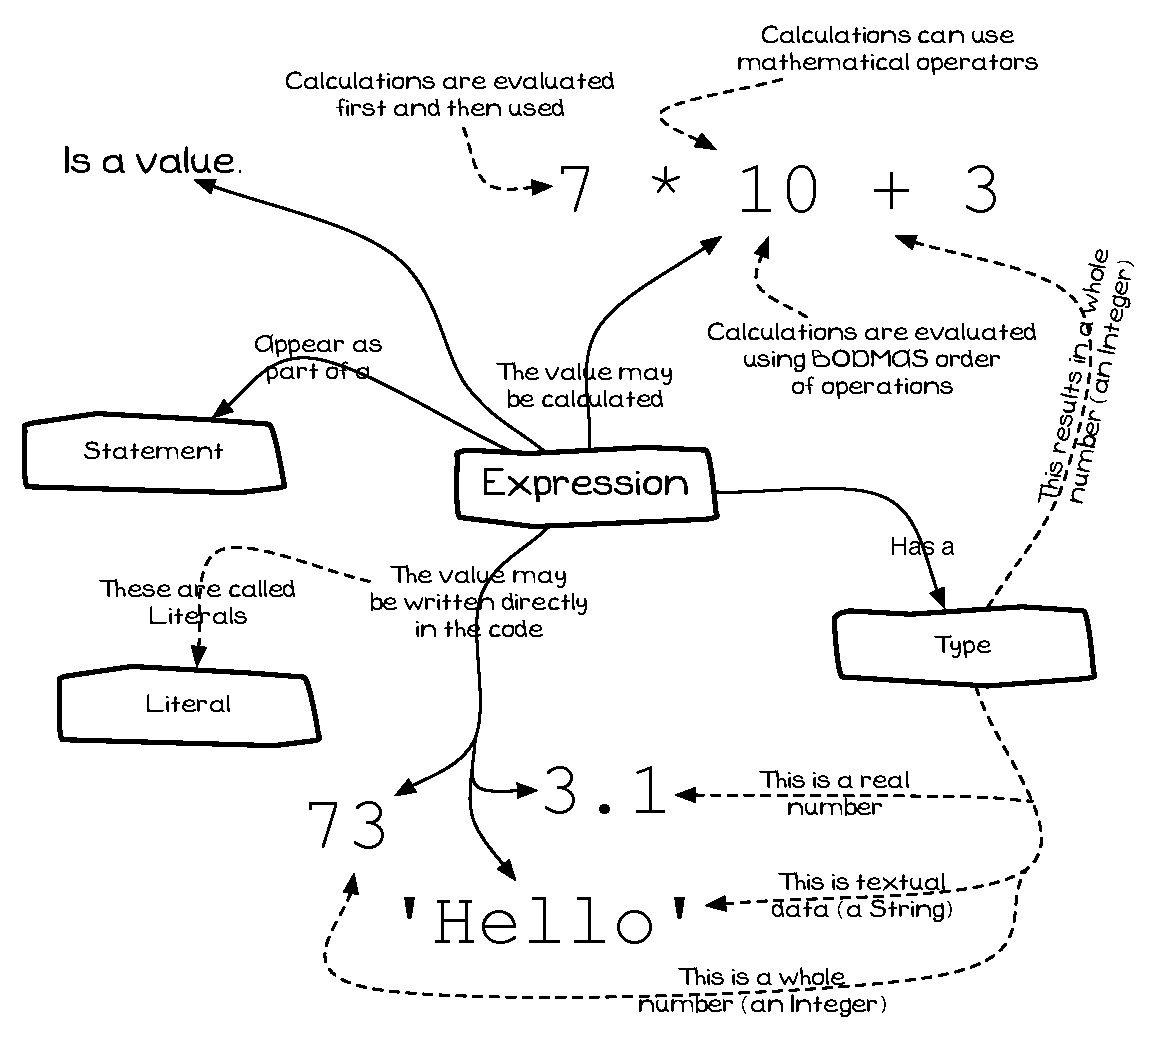
\includegraphics[width=\textwidth]{./topics/program-creation/diagrams/Expression} 
   \caption{An expression provides a \textbf{value} to be used in a Statement.}
   \label{fig:program-creation-expression}
\end{figure}


\mynote{
\begin{itemize}
  \item An expression is a \textbf{term} given to code that calculates a value.
  \item The concepts related to expressions are shown in Figure \ref{fig:program-creation-expression}.
  \item An expression provides a \textbf{value} that is used in a Statement.
  \item The expression's value may be calculated or entered directly into the code.
  \item Calculations can use mathematical operators: + for addition, - for subtraction, * for multiplication, $/$ for division, and parenthesis ( ) for grouping.
  \item Expressions are evaluated using the BODMAS\footnote{BODMAS indicates that expressions are evaluated \textbf{B} brackets first, \textbf{O} orders (which includes powers and square roots), \textbf{DM} for division and multiplication (which are of equal precedence, and are evaluated left-to-right), then \textbf{AS} addition and subtraction (of equal precedence, evaluated left-to-right).} order of operations.
  \item Values entered directly within an expression are \textbf{Literal} values.
\end{itemize}
}

% section program (end)